% Propósito: ubicar las estructuras principales del oído externo, medio e
% interno y mostrar la continuidad de la vía aérea hasta la cóclea.
% Origen: descripción anatómica funcional de las secciones
% \ref{sec:u6-oido-externo}, \ref{sec:u6-anatomia-oido-medio} y
% \ref{sec:u6-rampas-fluidos}. Esquema propio, simplificado y sin escala.
% Descripción accesible: de izquierda a derecha se observan el pabellón y el
% canal auditivo externo, la membrana timpánica, los tres huesecillos, las
% ventanas oval y redonda y una cóclea en espiral. Una rama inferior representa
% la trompa de Eustaquio. Fondos grises separan oído externo, medio e interno.
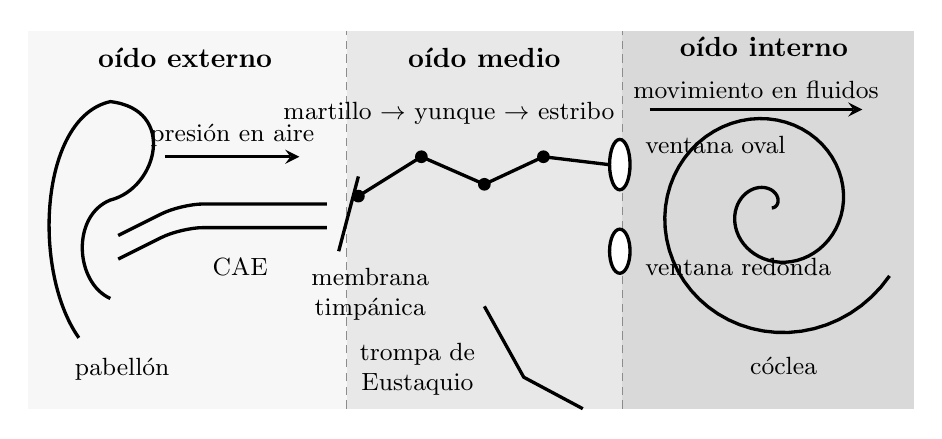
\begin{tikzpicture}[font=\small,>=stealth,x=1cm,y=1cm]
    \fill[black!3] (0.10,0.35) rectangle (4.15,5.15);
    \fill[black!9] (4.15,0.35) rectangle (7.65,5.15);
    \fill[black!15] (7.65,0.35) rectangle (11.35,5.15);
    \draw[densely dashed,black!45] (4.15,0.35) -- (4.15,5.15);
    \draw[densely dashed,black!45] (7.65,0.35) -- (7.65,5.15);

    \node[font=\bfseries] at (2.10,4.80) {oído externo};
    \node[font=\bfseries] at (5.90,4.80) {oído medio};
    \node[font=\bfseries] at (9.45,4.95) {oído interno};

    % Pabellón y canal auditivo externo.
    \draw[very thick]
        (0.75,1.25) .. controls (0.15,2.10) and (0.25,4.05) .. (1.15,4.25)
        .. controls (2.00,4.15) and (1.75,3.15) .. (1.15,3.00)
        .. controls (0.65,2.80) and (0.70,1.95) .. (1.15,1.75);
    \draw[very thick,rounded corners=8pt]
        (1.25,2.55) -- (2.05,2.95) -- (3.90,2.95);
    \draw[very thick,rounded corners=8pt]
        (1.25,2.25) -- (2.05,2.65) -- (3.90,2.65);
    \node[align=center] at (1.30,0.85) {pabellón};
    \node[align=center] at (2.80,2.15) {CAE};

    % Membrana timpánica y cadena osicular.
    \draw[very thick] (4.05,2.35) -- (4.30,3.30);
    \node[align=center] at (4.45,1.80) {membrana\\timpánica};
    \draw[very thick] (4.30,3.05) -- (5.10,3.55) -- (5.90,3.20)
        -- (6.65,3.55);
    \fill (4.30,3.05) circle (2.3pt);
    \fill (5.10,3.55) circle (2.3pt);
    \fill (5.90,3.20) circle (2.3pt);
    \fill (6.65,3.55) circle (2.3pt);
    \node[align=center] at (5.45,4.10) {martillo \(\rightarrow\) yunque
        \(\rightarrow\) estribo};
    \draw[very thick] (6.65,3.55) -- (7.48,3.45);

    % Ventanas, cóclea y trompa.
    \draw[very thick,fill=white] (7.62,3.45) ellipse (0.13 and 0.32);
    \draw[very thick,fill=white] (7.62,2.35) ellipse (0.13 and 0.28);
    \node[anchor=west] at (7.82,3.70) {ventana oval};
    \node[anchor=west] at (7.82,2.15) {ventana redonda};

    \draw[very thick]
        plot[domain=0:690,samples=120]
        ({9.55+0.0025*\x*cos(\x)},{2.90+0.0025*\x*sin(\x)});
    \node at (9.70,0.90) {cóclea};

    \draw[very thick] (5.90,1.65) -- (6.40,0.75) -- (7.15,0.35);
    \node[align=center] at (5.05,0.85) {trompa de\\Eustaquio};

    \draw[->,very thick] (1.85,3.55) -- (3.55,3.55)
        node[midway,above] {presión en aire};
    \draw[->,very thick] (8.00,4.15) -- (10.70,4.15)
        node[midway,above] {movimiento en fluidos};
\end{tikzpicture}
